\documentclass[12pt]{article}

\usepackage[utf8]{inputenc}
\usepackage[T1]{fontenc}
\usepackage{datetime}
\usepackage[spanish]{babel}
\usepackage{graphicx}
\usepackage{listings}
\usepackage{caption}
\usepackage{subcaption}
\usepackage[right=2cm,left=2cm,top=2cm,bottom=2cm]{geometry}
\usepackage{hyperref}
\usepackage{fancyhdr}
\usepackage{color}
\usepackage[export]{adjustbox}
\usepackage{graphicx}
\usepackage{float}
\usepackage{changepage}
\usepackage{multicol}
\usepackage{imakeidx}
\usepackage{csquotes}
\usepackage{array}
\usepackage{tabularx}
\usepackage{xcolor}
\usepackage[backend=biber]{biblatex}
\addbibresource{webgrafia.bib}

\pagestyle{fancy}
\renewcommand{\footrulewidth}{0.4pt}
\setlength{\headheight}{15pt}


\fancyhead[L]{ CEIABD – SBD }
\fancyhead[R]{ Páez Anguita, Víctor }
\fancyfoot[L]{IES Gran Capitán}


\begin{document}

\begin{titlepage}
    \begin{center}
      \Large \bfseries{}
    \end{center}
    \vspace{0.1cm}
    \begin{center}
      \Large \bfseries{}
    \end{center}
    \vspace{0.1cm}
    \begin{center}
     \Large \bfseries{Pharma sales Dashboard}
    \end{center}
    \vspace{0.0001cm}
    \begin{center}
        Departamento de informática \\ I.E.S. Gran Capitán - Córdoba
    \end{center}
        \vspace{2 cm}
\begin{figure}[h!]
    \centering
    
\includegraphics[width=.6\textwidth]{assets/portada.png}
    \label{fig:my_label}
\end{figure}
    \vspace{0.2 cm}
    \begin{center}
        Inteligencia artificial y Big data \\ \today 
    \end{center}
    \vspace{4 cm}
\null\hfill \textbf{Desarrollado por:}
\\
\\
\null\hfill Víctor Páez Anguita
\clearpage
\end{titlepage}

%%%%%%%%%%%%%%%%%%%%%%%%%%%Index%%%%%%%%%%%%%%%%%%%%%%%%%%%%%%%%
\tableofcontents
\clearpage
%%%%%%%%%%%%%%%%%%%%%%%%%%%Index%%%%%%%%%%%%%%%%%%%%%%%%%%%%%%%%


\section{Pharma Sales}

El siguiente cuadro de mando de qlik controla las ventas de una empresa farmacéutica. En este se puede visualizar la evolución de las ventas, los productos más vendidos, 
aquellos asociados a los Rx total, farmaceuticos y sus ventas asociadas a productos de qlik y los que no y la evolución de las ventas por mes.
El cuadro de mando tiene tan solo 3 pestañas, pero cada una de ellas tiene una gran cantidad de información que se puede analizar y complejidad.

\subsection{Qlik Brands Performance}

En esta pestaña se puede visualizar la evolución de las ventas de los productos de la empresa farmacéutica.

\begin{figure}[h!]
    \centering
    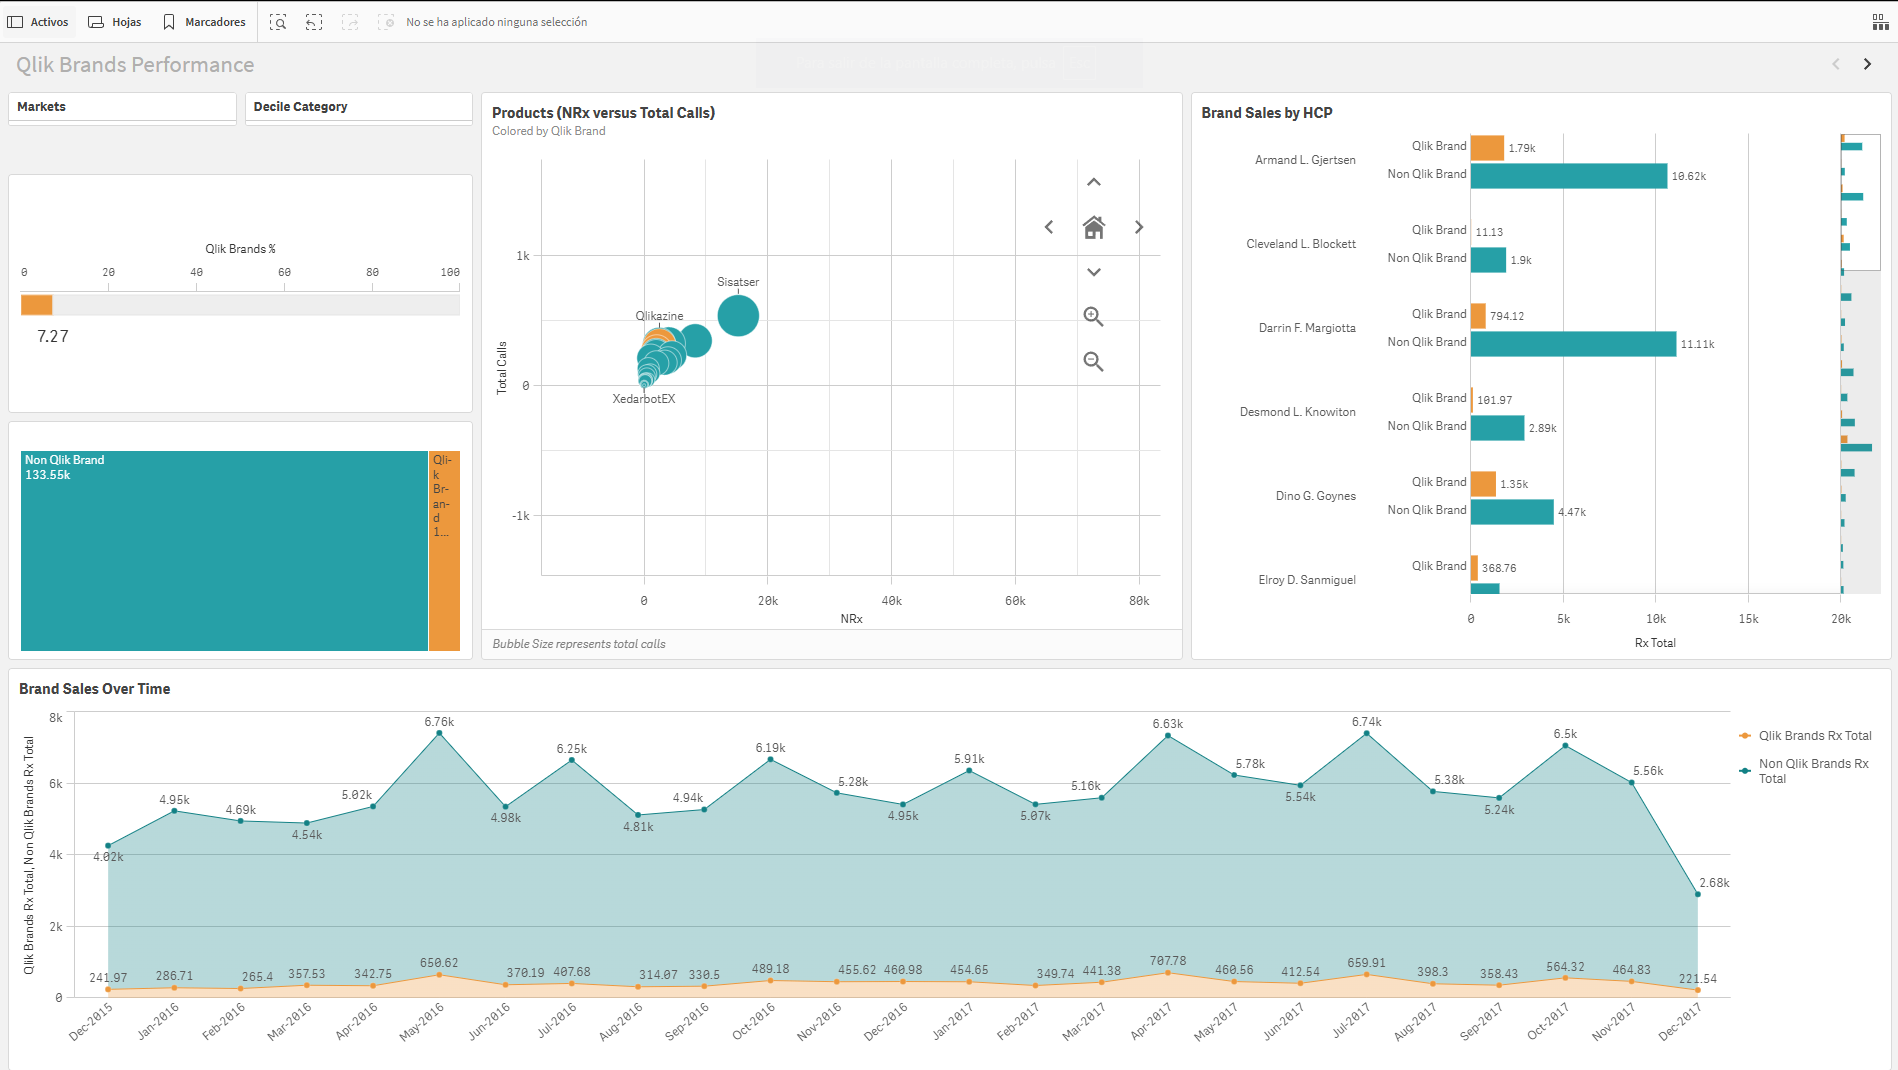
\includegraphics[width=.8\textwidth]{assets/qlik_1.PNG}
    \label{fig:my_label}
\end{figure}

Como podemos observar esta primera pestaña se divide en varias secciones. En la parte superior izquierda tenemos para segmentar
las ventas por mercado y categoría de la prescripción del producto. Seguido debajo tenemos un gráfico de barra único que indica
el porcentaje de presuspuesto de qlik que a tenido de ventas con respecto a los productos. Justo debajo podemos ver el gráfico
total de las ventas entre productos de qlik y no de qlik.
\\
En el centro podemos observar un gráfico de puntos en el que se calcula el total de llamadas de un podructo con respecto el volumen
de bolsa de la compañia NRx. Cada punto representa un producto y su tamaño indica el volumen de bolsa. Si hacemos click en cualquiera 
de ellos el cuadro de mando se ajustará para mostrar toda la información relacionada con ese producto.
\\
A la derecha podemos ver un gráfico de barras horizontal que muestra respecto a los HCP (responsables farmaceuticos de venta)
el total de ventas de los productos de qlik y no de qlik.
\\
Finalmente en la parte inferior podemos observar el gráfico más importante de la pestaña. El histórico de ventas de Qlik brand y 
no Qlik brand. En este gráfico podemos ver la evolución de las ventas de los productos de la empresa farmacéutica. (Desde 2015
hasta 2017).

\clearpage

\subsection{Prescriber Profile}

La siguiente pestaña esta más enfocada en los responsables farmaceuticos de venta.

\begin{figure}[h!]
    \centering
    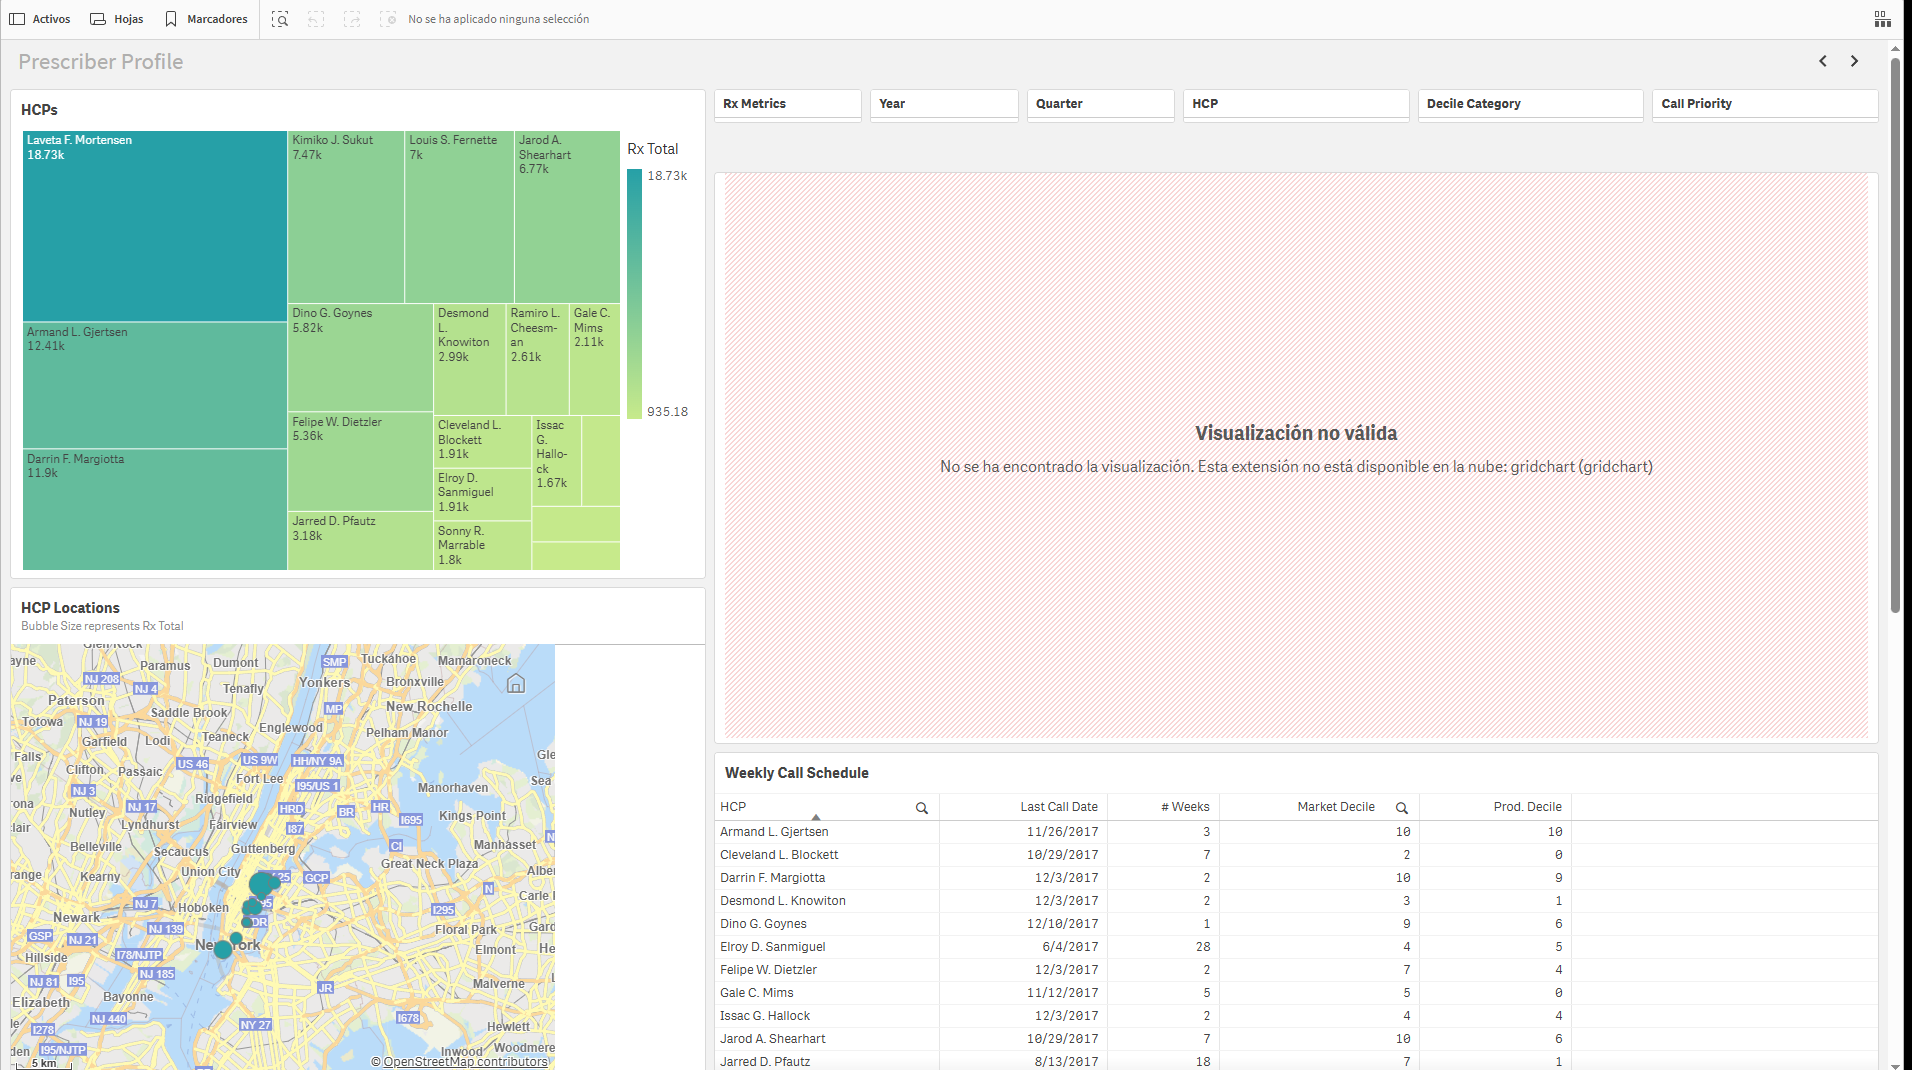
\includegraphics[width=.8\textwidth]{assets/qlik_2.PNG}
    \label{fig:my_label}
\end{figure}


En la parte superior izquierda tenemos un gráfico parecido a un mapa de calor que nos indica el total de ventas con respecto
a los responsables farmaceuticos de venta.
\\
Justo debajo podemos aprecir un mapa centrado en new york (de donde se sacan los datos de este cuadro) en el que se muestra
los puntos de venta de los productos de la empresa farmacéutica. Si hacemos click en cualquiera de estos puntos nos dará información
relativa a ese punto de venta.
\\
A la derecha tenemos una tabla de los HCP que nos muestra el número de llamadas, las semanas, el indicé del mercado y del producto.
\\
En la parte del medio izquierda tenemos un gráfico de barras horizontales de las llamadas a los productos con respecto al tiempo año/mes.
A la izquierda tenemos un gráfico de puntos con los meses más activos con respecto a los productos preescritos para los clientes.
\\
Finalmente en la parte inferior tenemos dos gráficos. A la izquierda uno de puntos y barras horizontales de un breakdown del mercado
con respecto a los productos y su Rx total (venta por volumen). A la derecha un gráfico de barras verticales representando el historico
del Rx total con respecto el tiempo.

\clearpage

\subsection{Product Profile}

La última pestaña probablemente es la más importante y útil. No solo tenemos una visualización completa si no que además
tenemos un buen filtro de busqueda.

\begin{figure}[h!]
    \centering
    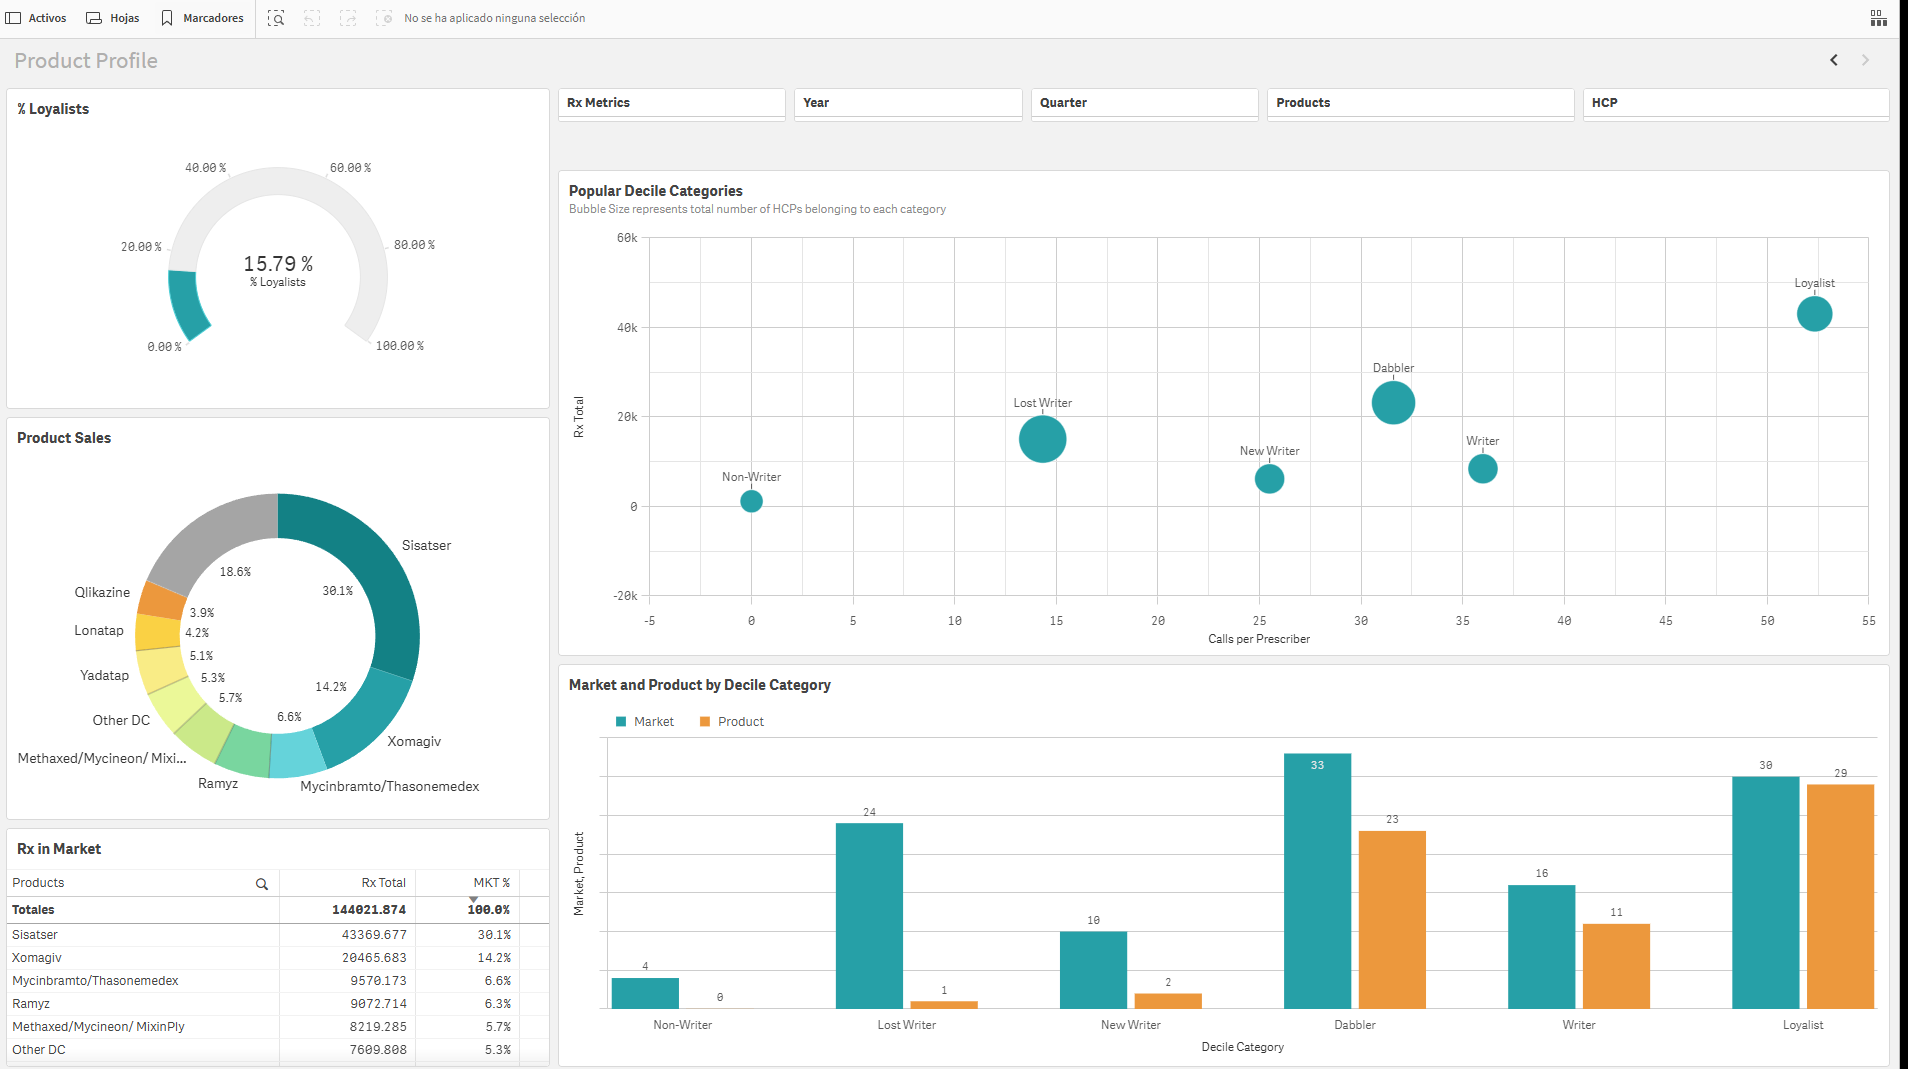
\includegraphics[width=.8\textwidth]{assets/qlik_3.PNG}
    \label{fig:my_label}
\end{figure}

Al principio podemos ver un gráfico de velocimetro que nos indica el porcentaje de lealtad con respecto a la preescripción del producto.
\\
Tenemos también un gráfico de tarta donde podemos ver el porcentaje de venta de los productos.
\\
Justo debajo tenemos una tabla que nos muestra información del Rx en el mercado.
\\
Si nos vamos a la derecha tenemos los filtros que podemos aplicar para la visualización y busqueda de los datos. Teniendo metricas de Rx,
año, cuartos del año, productos y responsables farmaceuticos de venta. Junto a un gráfico de puntos para visualizar mejors su busqueda.
\\
Finalmente en la parte inferior tenemos un gráfico de barras verticales que nos muestra la categoría de decimos de los productos y 
el mercado.

\clearpage

\section{Bibliografia}

\cite{Cuadro_de_mando}

\printbibliography

\end{document}
